\documentclass{beamer}
    \usetheme{Boadilla}
\usepackage{polyglossia}
    \setmainlanguage{english}
\usepackage{fontspec}
    \setsansfont{Linux Biolinum O}
\usepackage{graphicx}
\usepackage{xcolor} \usepackage{rotating}
\usepackage{listings}
    \lstset{language=bash,
	basicstyle=\footnotesize\ttfamily\tiny,
	breaklines=true,
	framextopmargin=50pt,
	frame=bottomline,
	backgroundcolor=\color{white!86!black},
	commentstyle=\color{blue},
	keywordstyle=\color{red},
	stringstyle=\color{orange!80!black}}
\usepackage{amsmath}
\usepackage{amssymb}
\usepackage[binary-units=true]{siunitx}
\usepackage{booktabs}
\usepackage{float}
\usepackage{tabularx}
\usepackage{caption}
\usepackage{subfig}
\usepackage{tikz}
    \usetikzlibrary{patterns}
    \usetikzlibrary{decorations.pathreplacing}
\usepackage{datenumber}
\setbeamertemplate{itemize items}[circle]
\usepackage{hyperref}
     \hypersetup{
     colorlinks=true,
     linkcolor=black,
     filecolor=magenta}

\title{\texorpdfstring{\color{blue!50!black}\textbf{Cosmics with ALPIDE}}{}}
\subtitle{Bachelor Student Report}
\author[Maurice \and David]{Maurice Donner \and David Schledewitz}
\date{September 22th, 2020}

\begin{document}

\maketitle
\newpage

%\begin{frame}{The Telescope}
%    \begin{figure}[H]
%	\centering
%	%\includegraphics[width=\textwidth]{%TODO HIER REIN} %MENTION WHO YOU ARE AND INTRODUCE
%    \end{figure}
%\end{frame}

\begin{frame}{First Steps}
    \begin{itemize}
	\item Started working in May
	\item Limited access to GSI
	\item Set up the telescope to be pointed towards the sky and record
	    cosmics
	\item At first \textbf{no scintillators} available \\[1cm]
    \end{itemize}

\LARGE Method of operation \footnotesize \\[.5cm]

\begin{minipage}[b]{.49\textwidth}
    \begin{itemize}
	\item Use a NIM pulse generator to create artificial triggers for the
	    chips.
	\item Trigger every \textasciitilde \( 100 \ \si{\micro \second} \) 
	    (when not busy).
	\item When discriminator signal and STROBE are in coincidence, event is
	    latched to memory
	\item That way no event should be missed
    \end{itemize}
\end{minipage}

    \begin{figure}[H]
    \centering \tiny
    \begin{tikzpicture}[remember picture, overlay,yshift=2cm,xshift=.5cm,scale=1.3]
    % Draw Coordinate system and axis labels
    \draw[->] (0,0) -- (4,0) node[anchor=north] {t};
    \draw[->] (0,0) -- (0,1);
    \draw (0,0) node[anchor=north] {0 $\si{\micro \second}$};
    \draw (2,0) node[anchor=north] {95.8 $\si{\micro \second}$};
    % Draw Strobes
    \filldraw[fill=blue!20,draw=blue!50!black] (0,0) rectangle (1.8,0.8);
    \filldraw[fill=blue!20,draw=blue!50!black] (2,0) rectangle (3.8,0.8);
    % Draw strobe length
    \draw [decorate,decoration={brace,amplitude=3pt},xshift=0pt,yshift=1pt]
    (2.0,0.8) -- (3.8,0.8) node [black,midway,yshift=10pt] 
    {$90 \ \si{\micro \second}$ };
    % Draw Discriminator Signal
    \draw[pattern=north west lines,pattern color = red!50!black] (1.9,0) rectangle (2.1,0.8);
    \draw[pattern=north west lines,pattern color = red!50!black] (0.4,0) rectangle (0.6,0.8);
    % Draw discriminator signal length
    \draw [decorate,decoration={brace,amplitude=1pt},xshift=0pt,yshift=1pt]
    (0.4,0.8) -- (0.6,0.8) node [black,midway,yshift=5pt] 
    {$10 \ \si{\micro \second}$ };
    % Draw Legend
    \filldraw[fill=blue!20,draw=blue!50!black] (0,-0.4) rectangle (0.2,-0.6)
    node[anchor=west] {STROBE signal};
    \draw[pattern=north west lines,pattern color = red!50!black] (0,-0.8) rectangle (0.2,-1)
    node[anchor=west] {Discriminator signal};
    % Draw Trigger
    \draw[->] (2.0, 1.1) -- (2.0, 0.9) node[anchor=south,yshift=5pt] {\tiny trigger};
    \end{tikzpicture}
    \end{figure}
\end{frame}

\begin{frame}{First Steps}
    \Large PROs \footnotesize \\
    \begin{itemize}
	\item Running "without" external trigger possible
	\item Uptime is close to 100\%
	\item Telescope can (and had) be operated \textbf{REMOTELY}
	\item Thin time slices makes it really unlikely to detect
	    two muons at the same time, especially from similar angles. \\[.5cm]
    \end{itemize}
    \Large CONs \footnotesize 
    \begin{itemize}
	\item $> 10 \, 000$ Events per second (mostly empty)
	\item $4.4 \ \si{\mega \byte}$ per second of Data written to the disk
	\item EUDAQ 1 crashed often at filesizes \( > 5 \ \si{\giga \byte} \)
	    $\rightarrow$ Runtime limited to \( \approx 18 \ \si{\minute} \) 
    \end{itemize} 
\end{frame}

\begin{frame}{Taking Cosmics} 
    Took 380 runs á 14-18 minutes in total over the course of several weeks
    \begin{figure}[H]
	\centering
	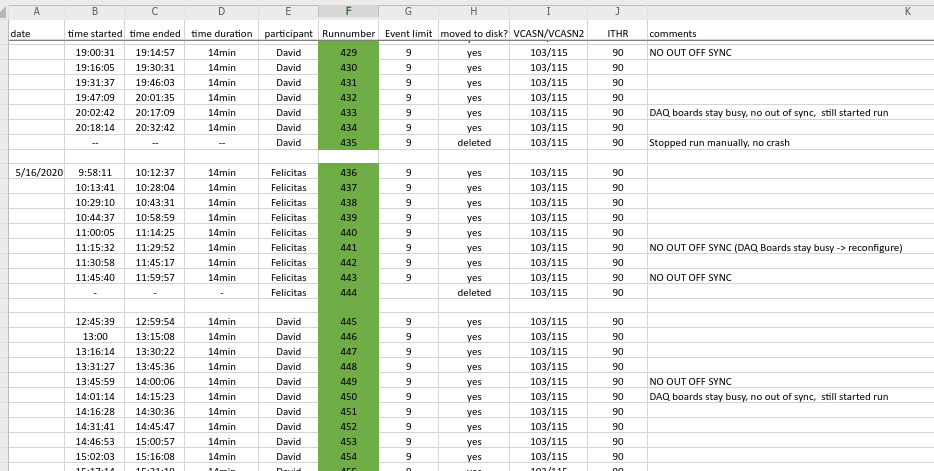
\includegraphics[width=.9\textwidth]{Screenshot.png}
    \end{figure}
    \footnotesize
    \begin{minipage}{.33\textwidth}
	\begin{itemize}
	    \item 1.5 TB of Data
	\end{itemize}
    \end{minipage}
    \begin{minipage}{.65\textwidth}
	\begin{itemize}
	    \item First analysis showed only \textasciitilde 10 good tracks
	       per run
	\end{itemize}
    \end{minipage}
\end{frame}

\begin{frame}[fragile]{Cosmic Analysis}
    \footnotesize
    \begin{itemize}
	\item Corryvreckan fails to do analysis with just a few tracks per run \\
	    \tiny (no way of combining multiple \verb`.raw` files for alignment?)
	    \footnotesize
	\item Used the \verb`[TextWriter]` module to transform RAW data into 
	    \verb`.txt` files.
	    \begin{itemize} 
		    \tiny \item Reducing filesize from \textasciitilde \( 4.5 \ \si{\giga \byte} \)
		    to \textasciitilde \( 200 \ \si{\mega \byte} \) per run \footnotesize
	    \end{itemize} 
	\pause
	\item Compression program stores only non-empty events.
	    \begin{itemize}
		    \tiny \item Reduces size of \verb`.txt` files to \textasciitilde
		    \( 90 \ \si{\kilo \byte} \) (Only non-empty events) \footnotesize
	    \end{itemize}
	\item Further analysis in Python
    \end{itemize}
\end{frame}

\begin{frame}{Cosmic Analysis}
    \footnotesize
    \begin{itemize}
	\item First visualization attempts
	\item Plane alignment with testbeam data from 2019 \( \rightarrow \)
	    inaccurate \tiny (planes seem to have shifted) \footnotesize
    \end{itemize}
\begin{minipage}{.45\textwidth}
    \centering
    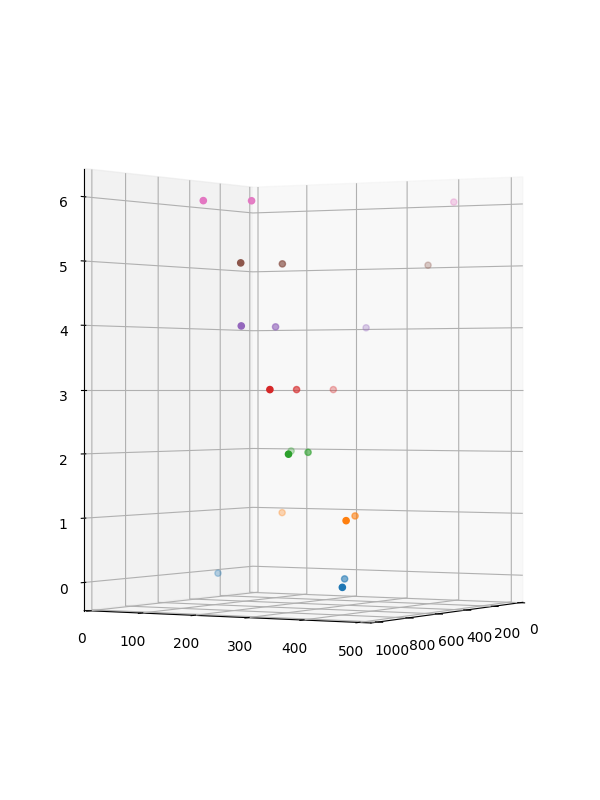
\includegraphics[trim=0 50 0 100,clip,width=\textwidth]{DESY_Before.png}
\end{minipage}
\begin{minipage}{.05\textwidth}
    \centering
    \( \rightarrow \) \\
    \tiny (align)
\end{minipage}
\begin{minipage}{.45\textwidth}
    \centering
    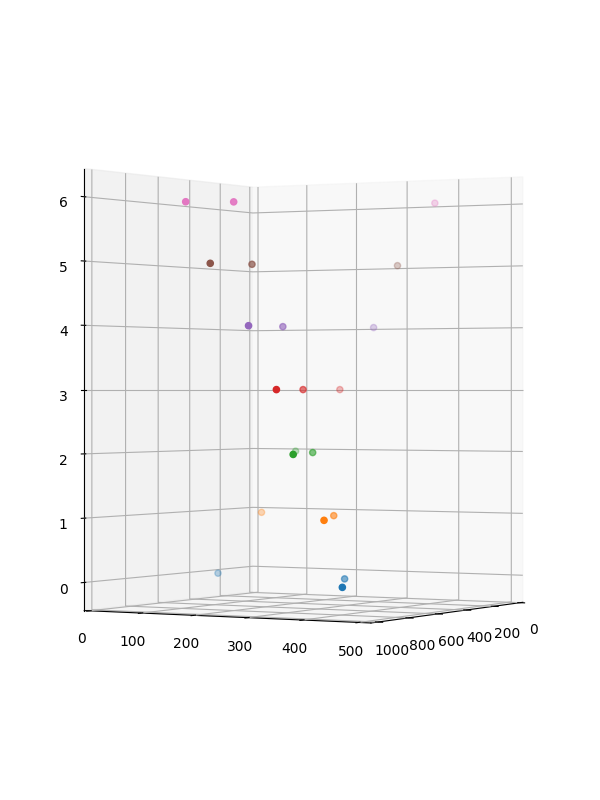
\includegraphics[trim=0 50 0 100,clip,width=\textwidth]{DESY_After.png}
\end{minipage}
\begin{itemize}
    \item Taking closer look at alignment
\end{itemize}
\begin{tikzpicture}[remember picture, overlay]
    \node[xshift=13,yshift=0,rotate=90] at (current page.center)
    {\tiny plane number};
    \node[xshift=-162,yshift=0,rotate=90] at (current page.center)
    {\tiny plane number};
    \node[xshift=60,yshift=-70,rotate=-2] at (current page.center)
    {\tiny Position [Pixel]};
    \node[xshift=-115,yshift=-70,rotate=-2] at (current page.center)
    {\tiny Position [Pixel]};
\end{tikzpicture}
\end{frame}

\begin{frame}{Cosmic Analysis}
    \footnotesize
    \begin{minipage}{.6\textwidth}
    \begin{figure}[H]
	\centering
	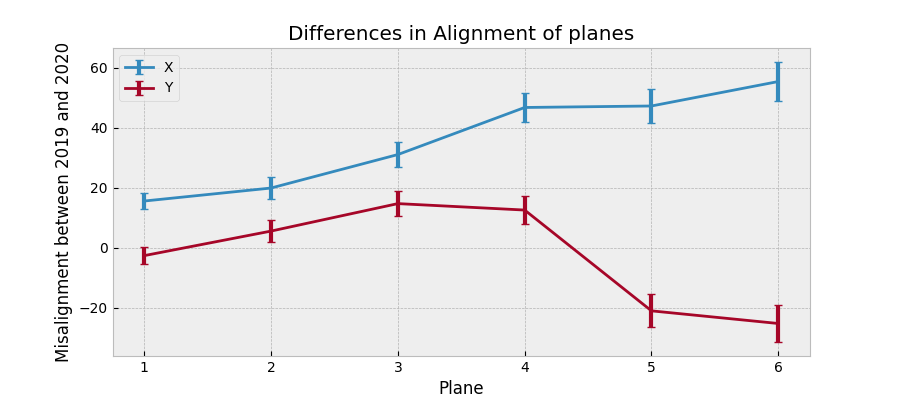
\includegraphics[trim=30 0 50 0, clip, width=\textwidth]{Misalignment.png}\\
	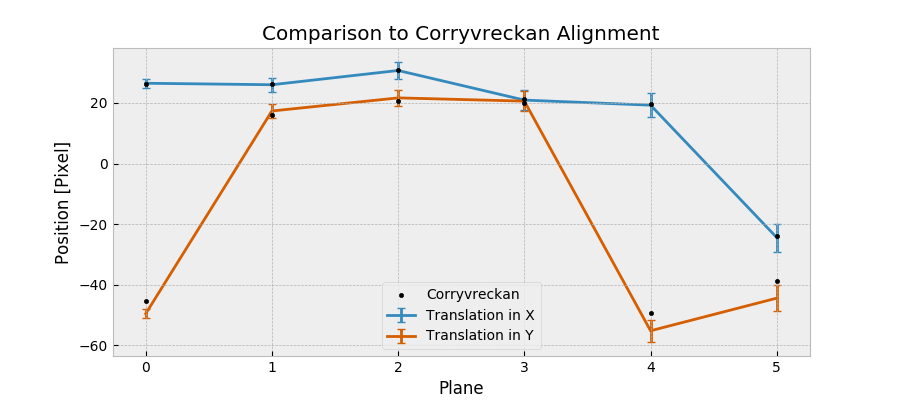
\includegraphics[trim=30 0 50 0, clip, width=\textwidth]{Corry.png}
    \end{figure}
    \end{minipage}
    \begin{minipage}{.39\textwidth}
	\begin{itemize}
	    \item First look at perpendicular tracks (testbeam)
	    \item Disalignment of planes to over \( 1.5 \ \si{\milli \meter} \)
		(after transport)
	    \item Generally, testbeam alignment from 2020 closer to cosmic
		setup than from 2019
	    \item Simple translation algorithm and comparison with the alignment
		that Corryvreckan suggests (second figure)
	    \item Goal: Do alignment with cosmic data \\[3pt] \tiny (new complication: angles)
	\end{itemize}
    \end{minipage}
\end{frame}

\begin{frame}[fragile]{Cosmic Analysis}
    Implemented a 3D-Fitting algorithm in Python:\\
    \begin{minipage}{.32\textwidth}
	\begin{figure}[H]
	    \centering
	    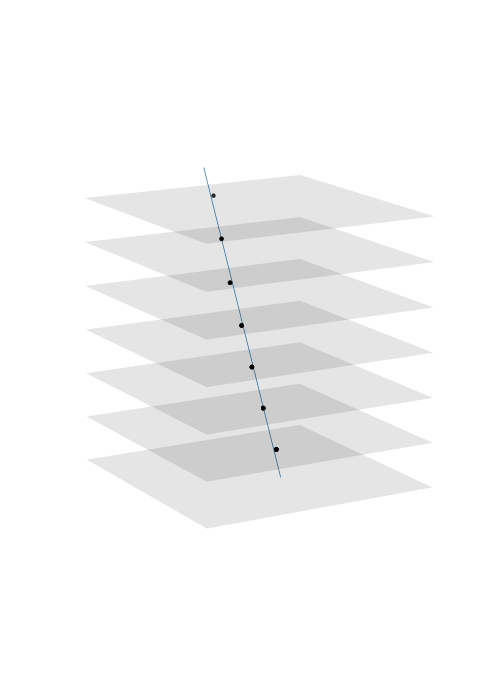
\includegraphics[trim=0 80 0 80,clip,width=\textwidth]{example_1459.png}
	\end{figure}
    \end{minipage}
    \begin{minipage}{.32\textwidth}
	\begin{figure}[H]
	    \centering
	    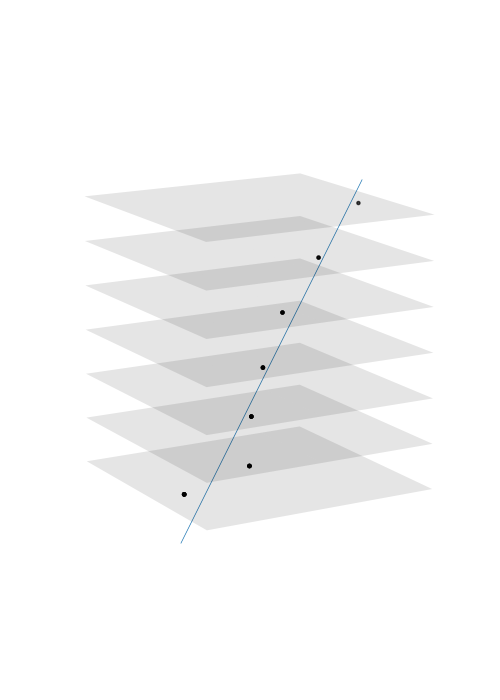
\includegraphics[trim=0 80 0 80,clip,width=\textwidth]{example_112000.png}
	\end{figure}
    \end{minipage}
    \begin{minipage}{.32\textwidth}
	\begin{figure}[H]
	    \centering
	    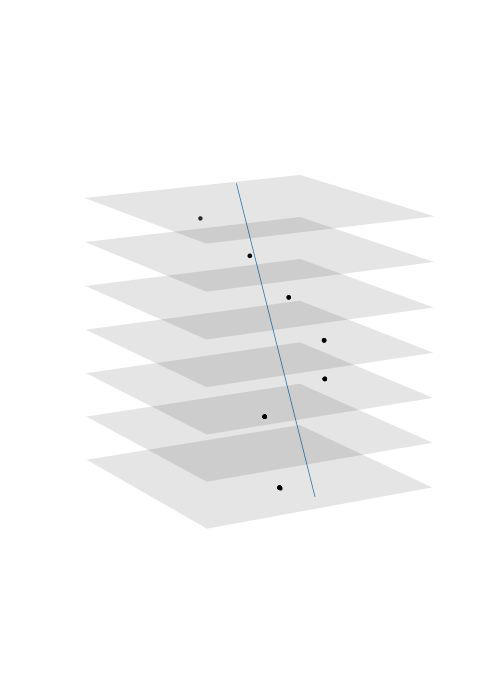
\includegraphics[trim=0 80 0 80,clip,width=\textwidth]{example_290252.png}
	\end{figure}
    \end{minipage}\\
    Using numpy's Singular value decomposition \verb]np.linalg.svd] \\[.1cm]
    \( \rightarrow \) Calculating \( \chi ^2 \) (goodness of fit) "by hand" \\
    \begin{minipage}{.4\textwidth}
	\begin{figure}[H]
	    \centering
	    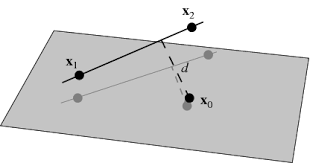
\includegraphics[width=\textwidth]{pointin3d.png}
	\end{figure}
    \end{minipage}
    \begin{minipage}{.59\textwidth}
	\footnotesize
	\begin{align*}
	    d^2 = \frac{ \left| x_1-x_0 \right|^2 \left| x_2-x_1 \right|^2
		- \left[ \left( x_1-x_0 \right) \cdot \left( x_2-x_1 \right)
		\right]^2}{\left| x_2-x_1 \right|^2}
	\end{align*}
    \end{minipage}\\[5pt]
\end{frame}

\sisetup{separate-uncertainty=true}

\begin{frame}{Event Analysis}
  \begin{itemize}
    \item Calculation of measurable muon rate
    \begin{itemize}
      \item Considering detector geometry, \\
      expected muon rate and angular distribution
    \end{itemize}
    \item Distinguish events by the number of traversed detector layers (planes)
    \begin{itemize}
      \item  Event with n traversed planes: n-plane-event (npE)
    \end{itemize}
  \end{itemize}
  \begin{center}
  \begin{tikzpicture}[scale=0.5]

    \draw[black, line width = 0.5mm] (-3,0) node[left] {6} -- (3,0);
    \draw[black, line width = 0.5mm] (-3,1.25) node[left] {5} -- (3,1.25);
    \draw[black, line width = 0.5mm] (-3,2.5) node[left] {4}-- (3,2.5);
    \draw[black, line width = 0.5mm] (-3,3.75) node[left] {3} -- (3,3.75);
    \draw[black, line width = 0.5mm] (-3,5) node[left] {2} -- (3,5);
    \draw[black, line width = 0.5mm] (-3,6.25) node[left] {1} -- (3,6.25);
    \draw[black, line width = 0.5mm] (-3,7.5) node[left] {0} -- (3,7.5);

    \draw[red, line width = 0.5mm] (-1.5,8.25) node[above] {\large 7pE} -- (1.5,-0.75);
    \draw[red, line width = 0.5mm] (0.5,8.25) node[above] {\large 6pE} -- (3.5,-0.75);
    \draw[red, line width = 0.5mm] (3.75,5.675) node[above right]{3pE} -- (-3.75,1.885);

  \end{tikzpicture}
  \end{center}
\end{frame}
\begin{frame}{Event Analysis}
  \begin{itemize}
    \item Comparison of evaluated data to expectation
  \end{itemize}
  \begin{figure}[H]
    \centering
    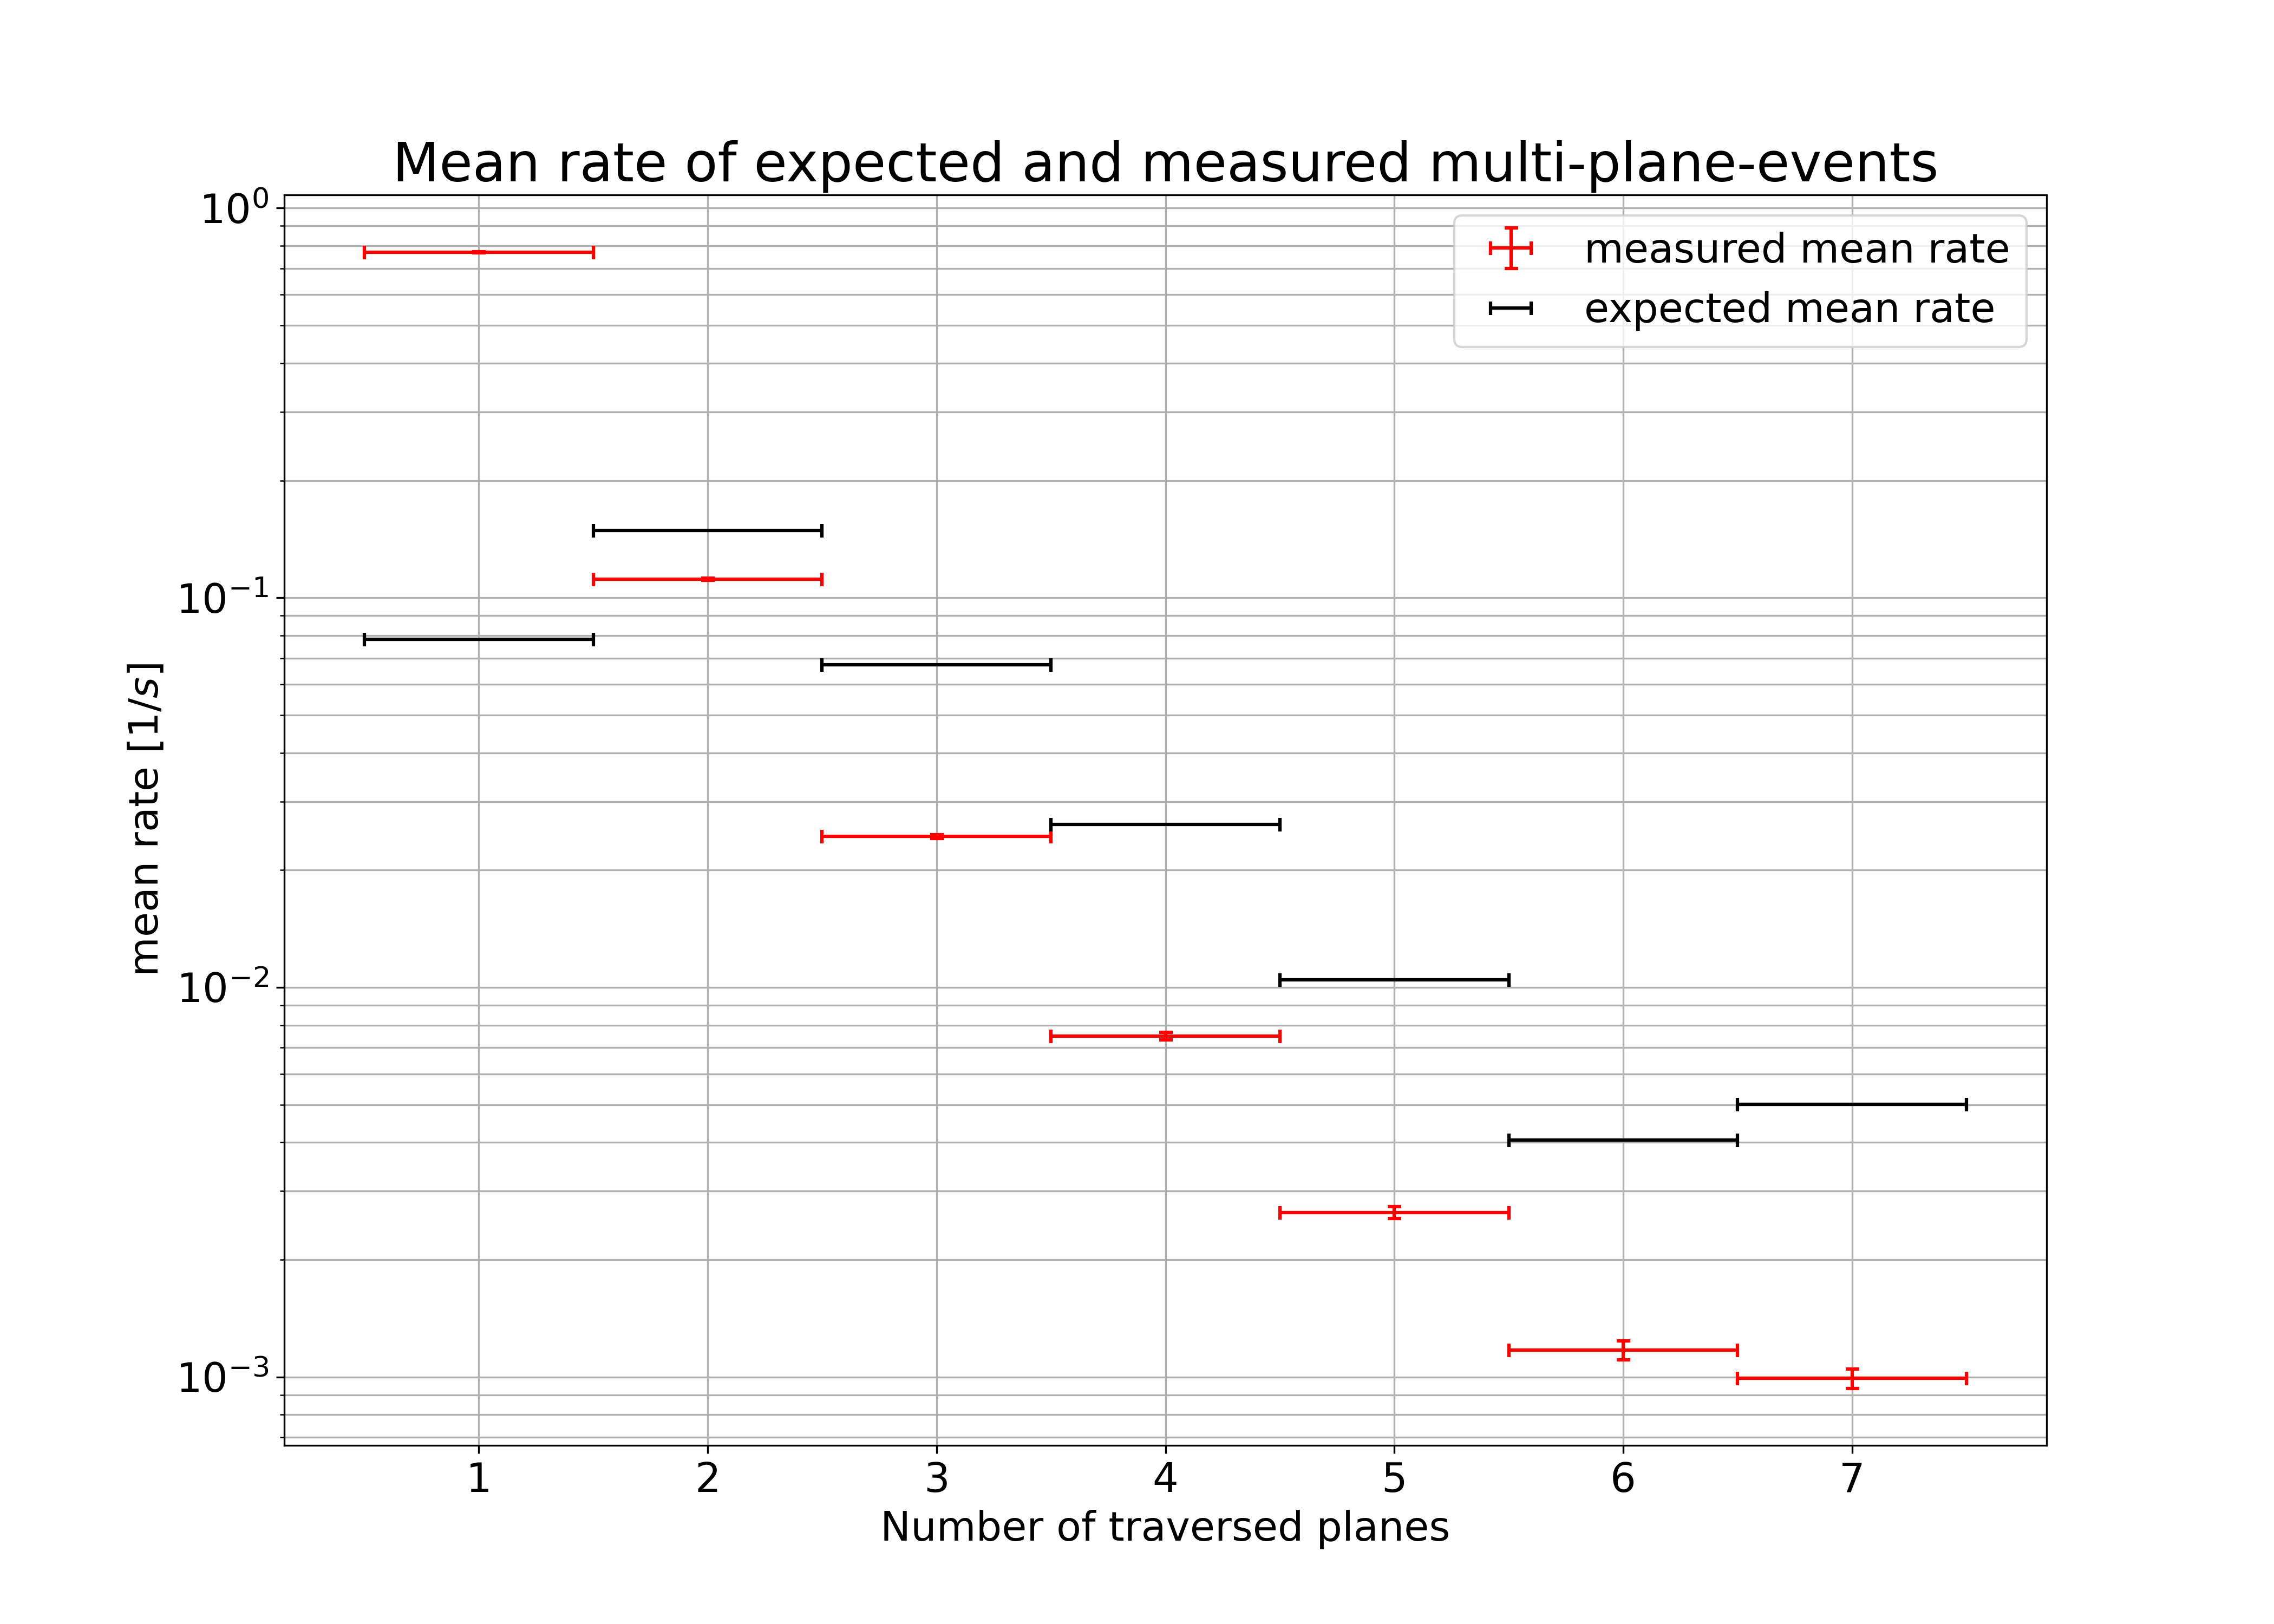
\includegraphics[width=.8\textwidth]{rate_comparison}
    %\caption{Comparison of estimated and measured muon rate}
  \end{figure}
  \begin{itemize}
	\item What are the reasons for the overestimation?
  \end{itemize}
\end{frame}

\begin{frame}{Event Analysis}
  \begin{itemize}
    \item Differences in measured mean hit rate per plane
    \item Dependency on thresholds
  \end{itemize}
  \begin{figure}[H]
    \centering
    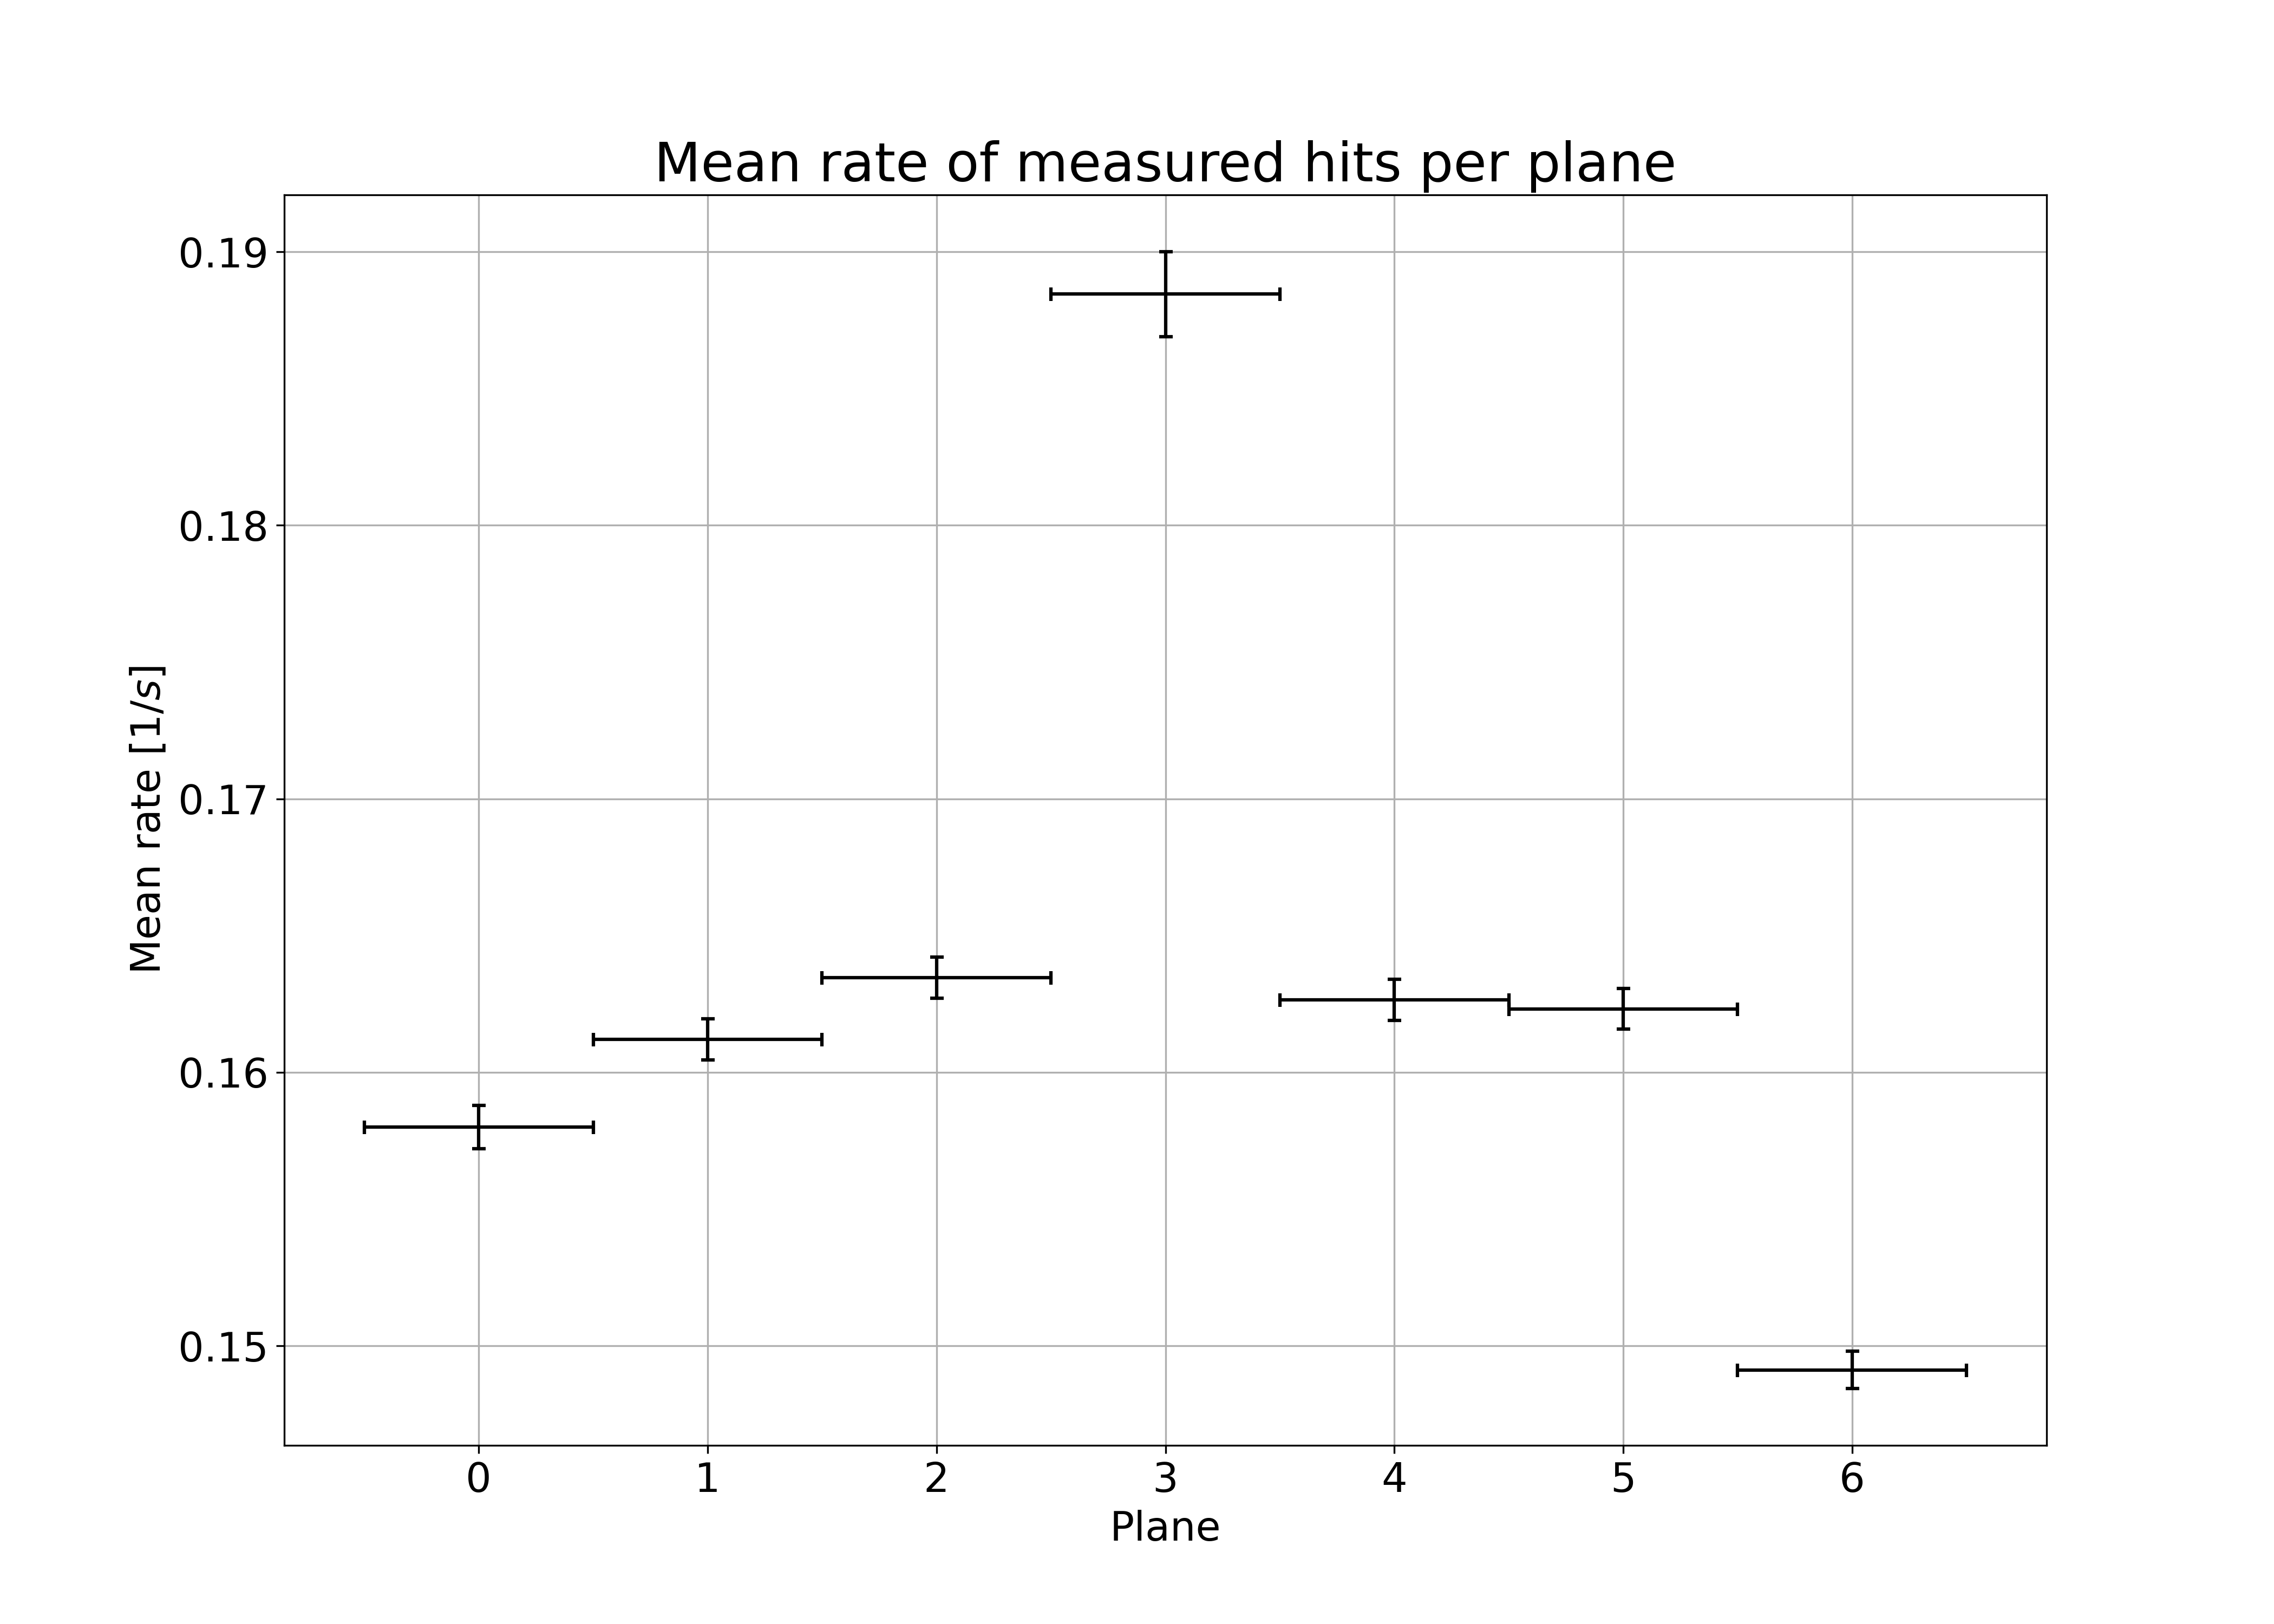
\includegraphics[width=.65\textwidth]{rate_per_plane}
    %\caption{Mean rate of measured hits}
  \end{figure}
  \begin{center}
  \resizebox{0.8\textwidth}{!}{%
  	\sisetup{table-figures-uncertainty=2,
  		table-figures-decimal=1,
  		table-number-alignment = center,
  		table-text-alignment = center}
  	%\centering
  	\begin{tabular}{cccccccc}
  		\toprule
  		Plane & 0 & 1 & 2 & 3 & 4 & 5 & 6 \\
  		\midrule
  		Threshold $[DAC]$ & 27.2(6) & 31.3(6) & 22.8(4) & 12.7(5) & 21.4(5) & 16.1(6) & 20.2(6) \\
  		\bottomrule
  	\end{tabular}
    %\caption{Thresholds of each plane}
  } % end of scope of "\resizebox"  directive
  \end{center}
\end{frame}

\begin{frame}{Event Analysis}
  \begin{itemize}
    \item Check for events with hits on not consecutive planes
    \begin{itemize}
      \item (i.e. planes 1,2,3,4,5,7 registering a hit lead to false 6pE)
    \end{itemize}
    \item Corrected mean rate by removing not consecutive plane events
    \item Further analysis with track information
  \end{itemize}
  \begin{figure}[H]
    \centering
    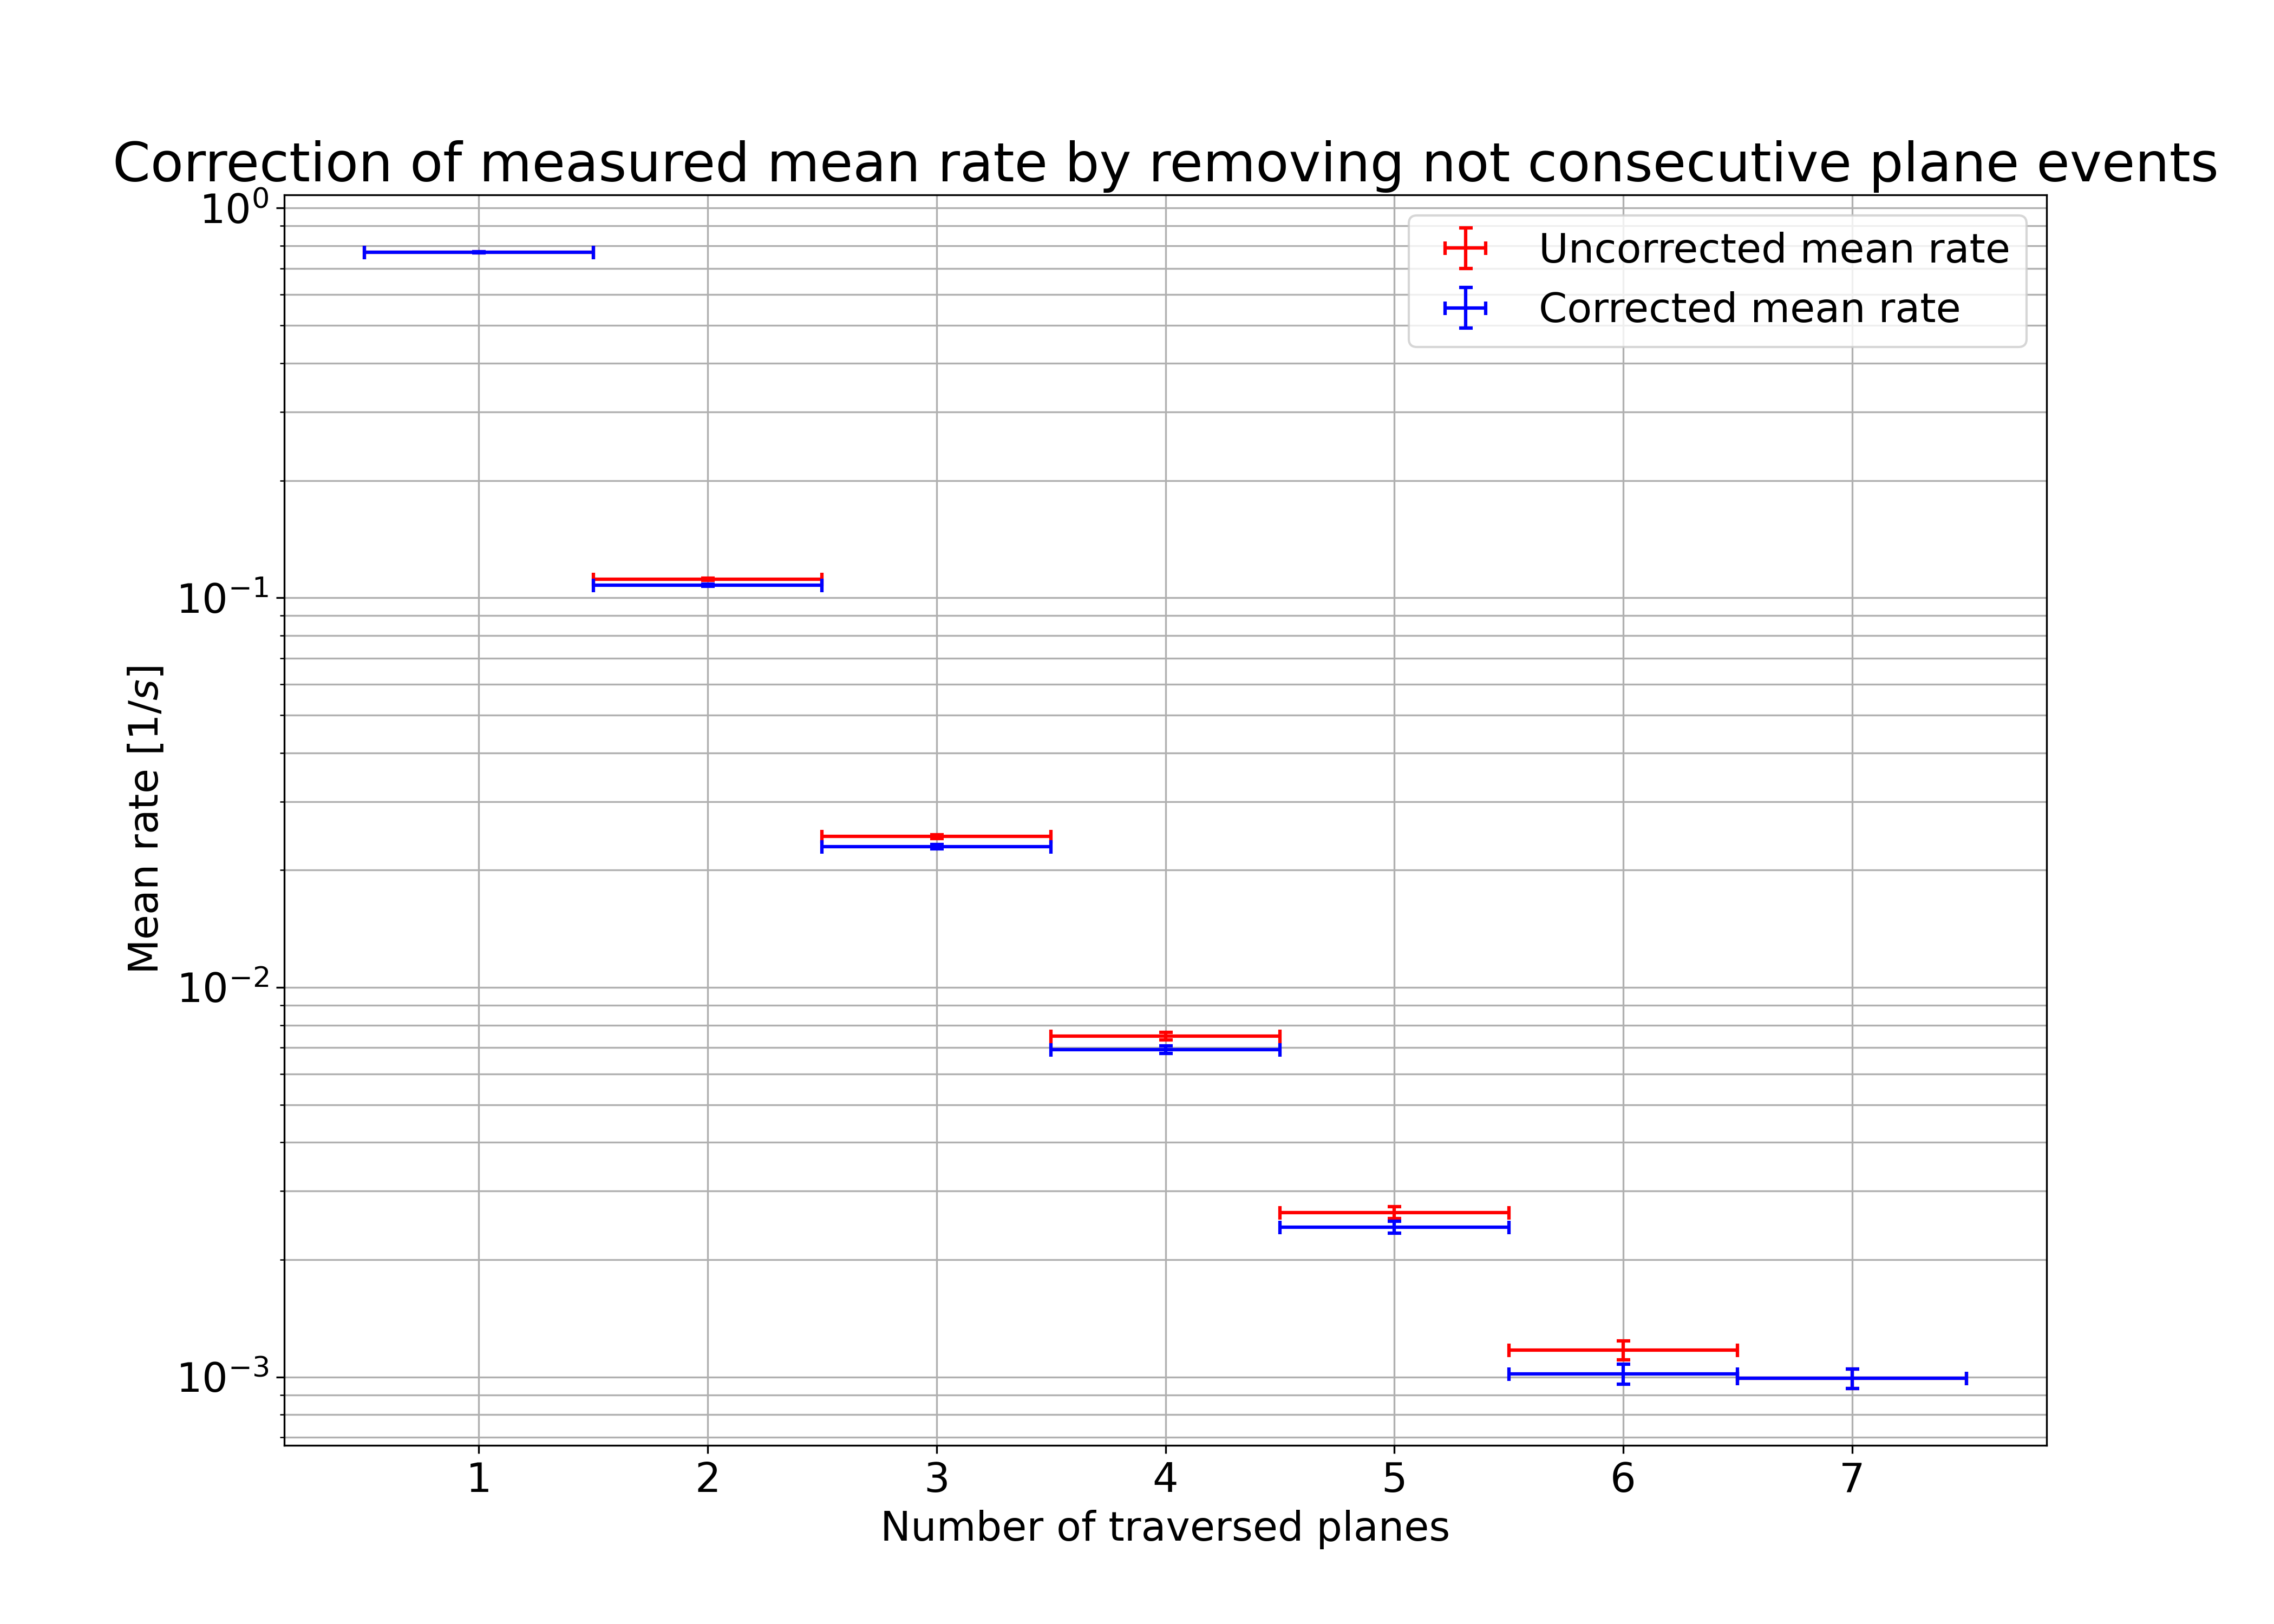
\includegraphics[width=.6\textwidth]{rate_correction}
    \caption{Mean rate correction by not consecutive plane events}
  \end{figure}
\end{frame}

\begin{frame}{Track Analysis}
  \begin{itemize}
    \item Track visualized with 2-dimensional projection
    \item Alignment with data of testbeam June 2020
    \item Possibility to classify events as valid or fake track
  \end{itemize}
  \begin{figure}[H]
    \centering
    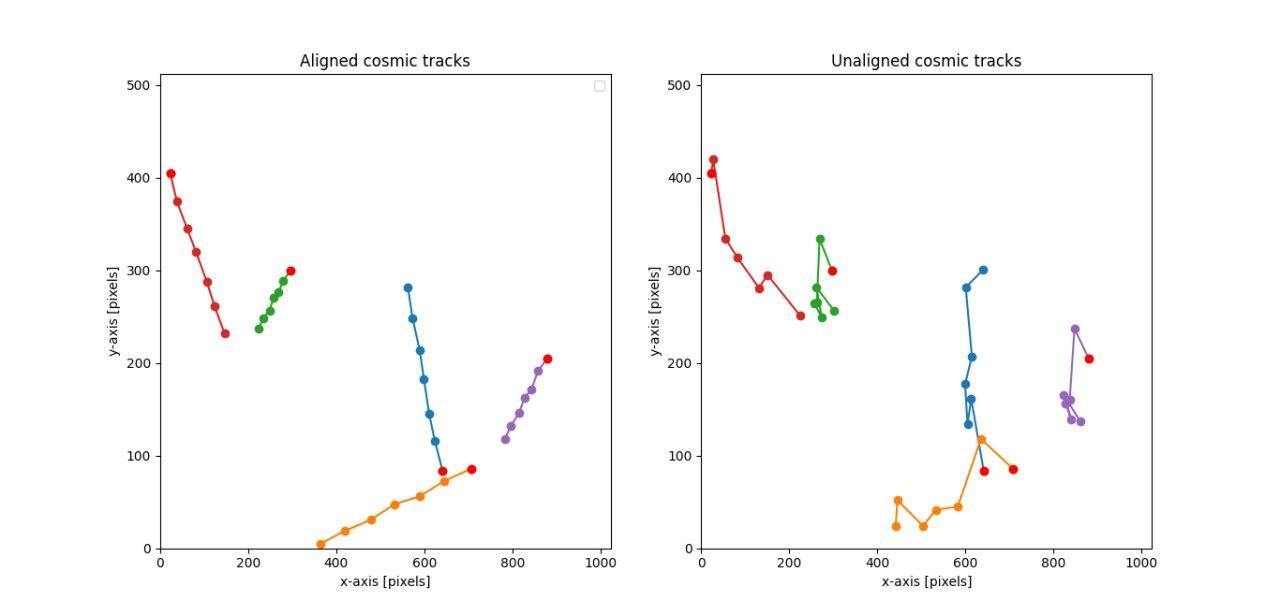
\includegraphics[width=.8\textwidth]{track_visual}
    \caption{Alignment with 2020 testbeam data}
  \end{figure}
\end{frame}

\begin{frame}{Track Analysis}
  \begin{itemize}
    \item Linear fit on 2D-track projections
    \item Analysis of $\chi^2_{red}$-distribution and angular distribution
    \item Open questions regarding the angular distribution (e.g. too few entries at small angles)

  \end{itemize}
  \begin{figure}[H]
    \centering
    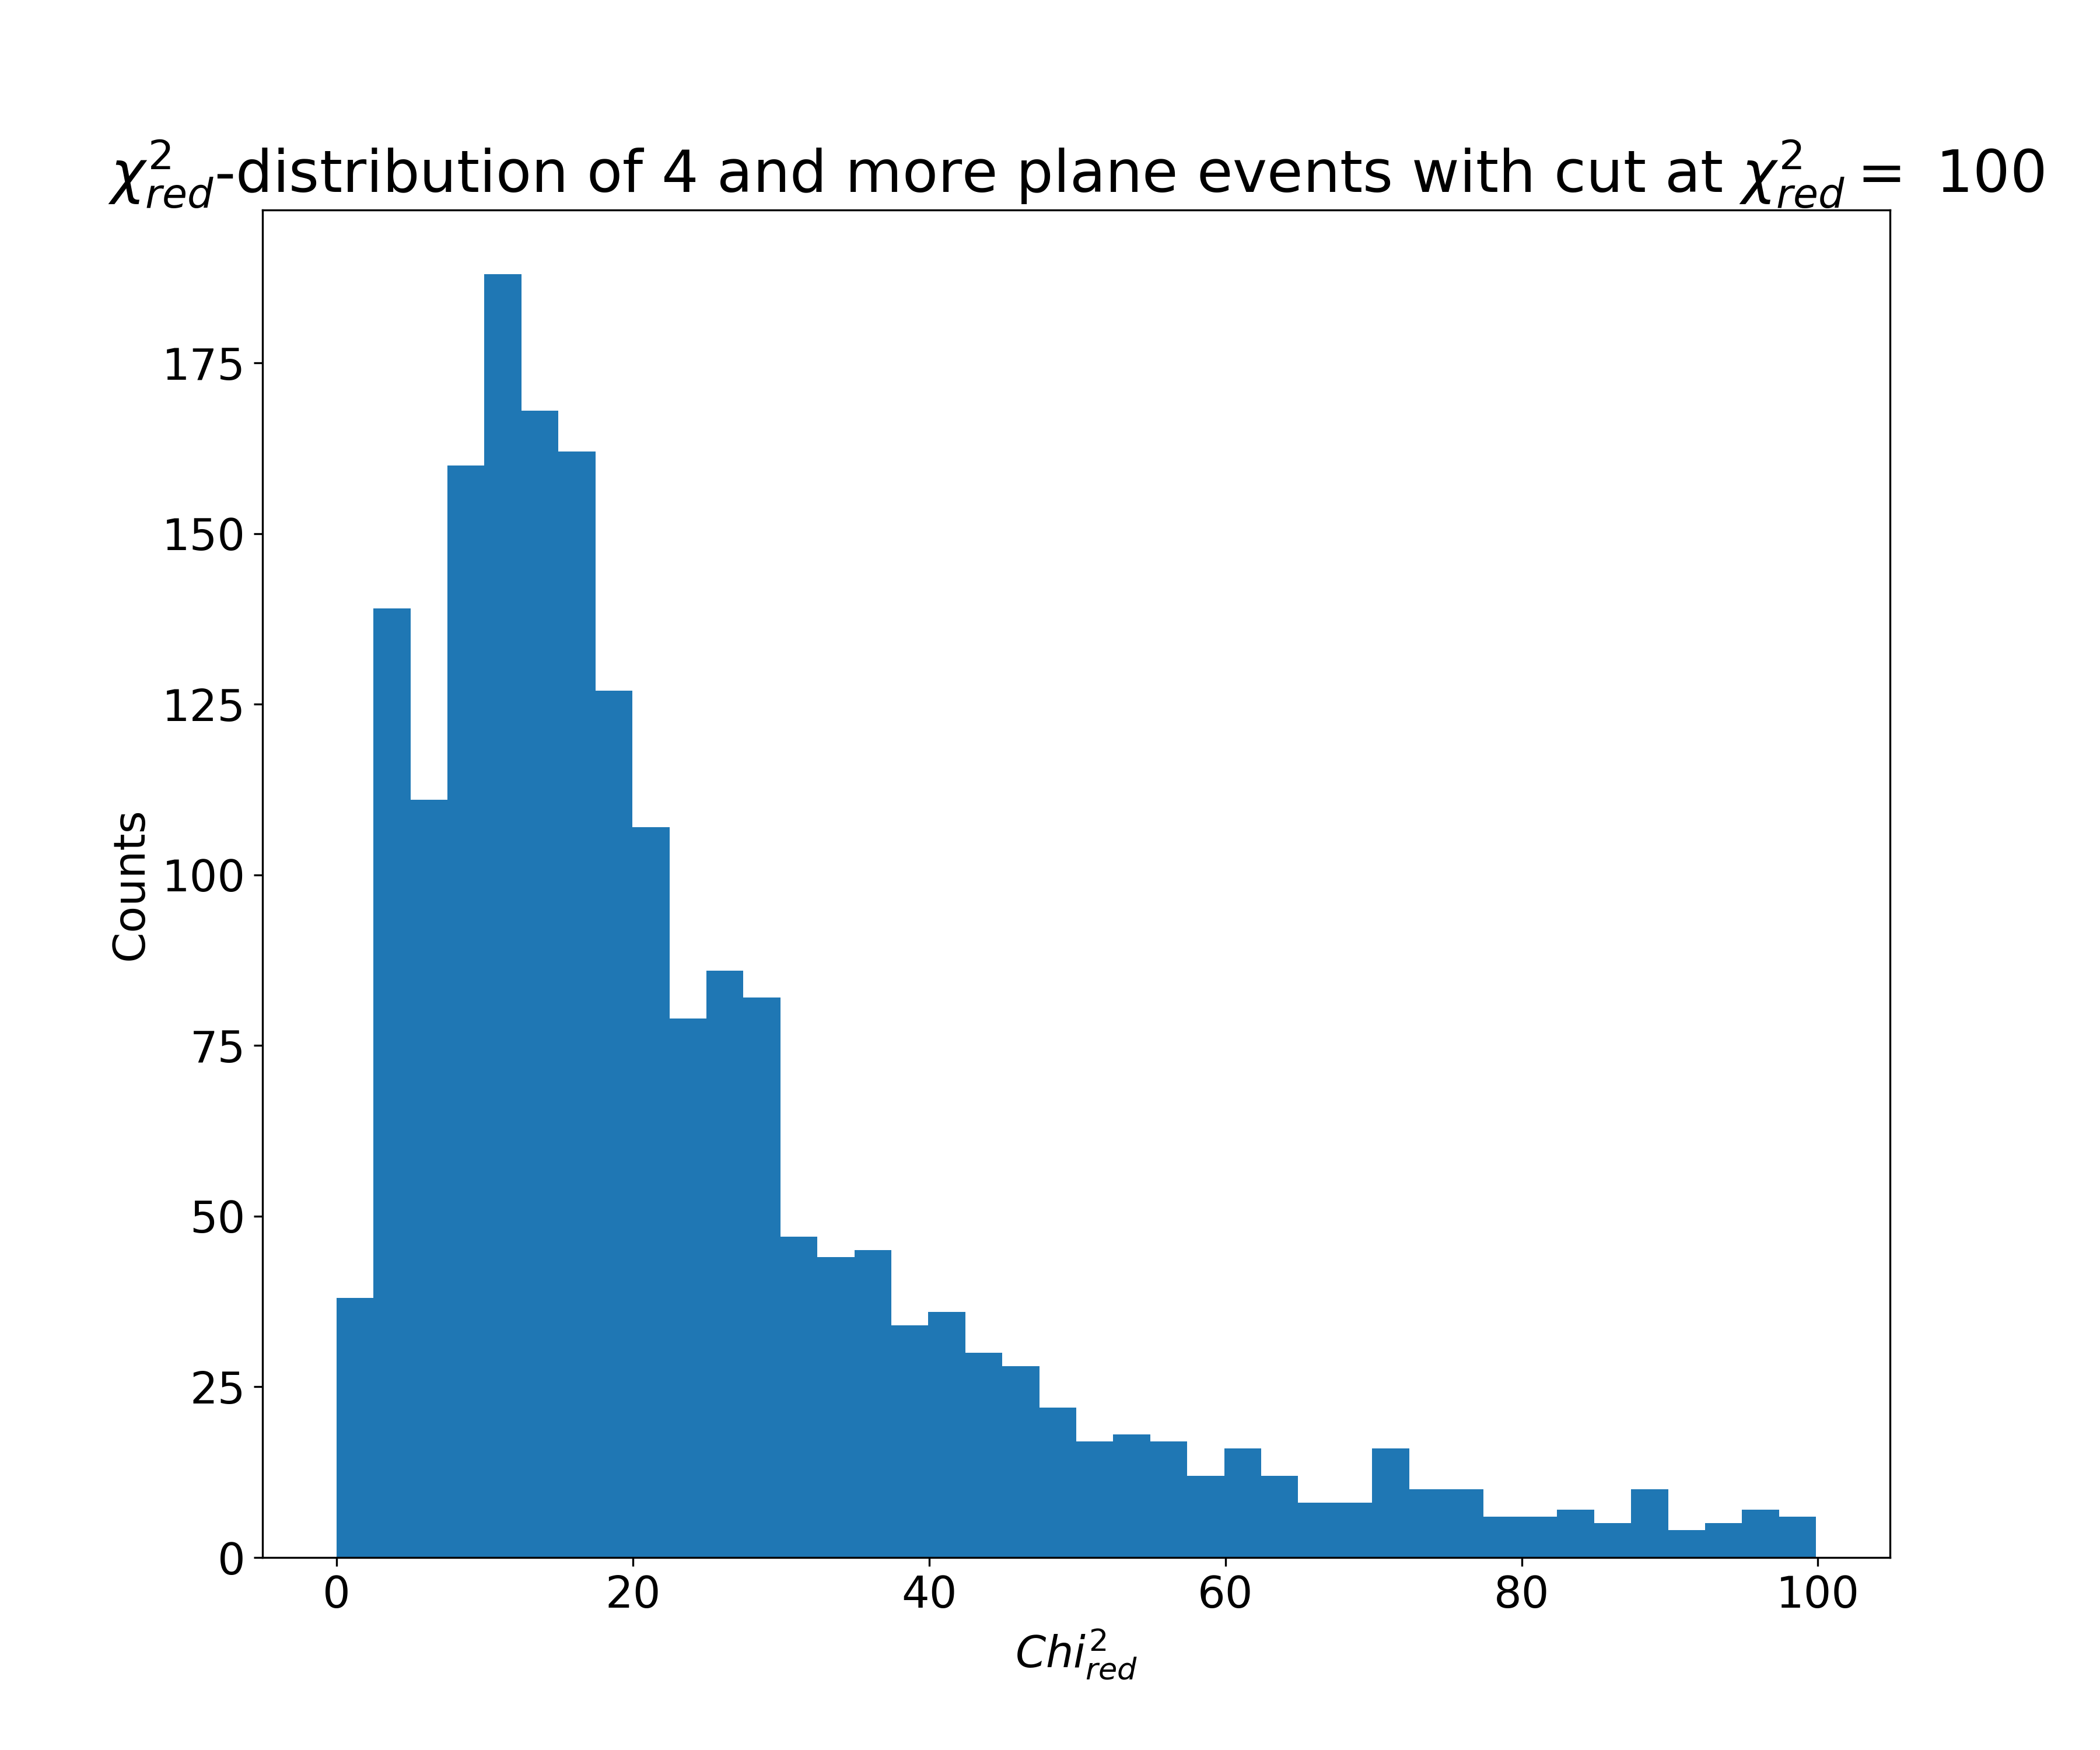
\includegraphics[width=.49\textwidth]{track_chi}
    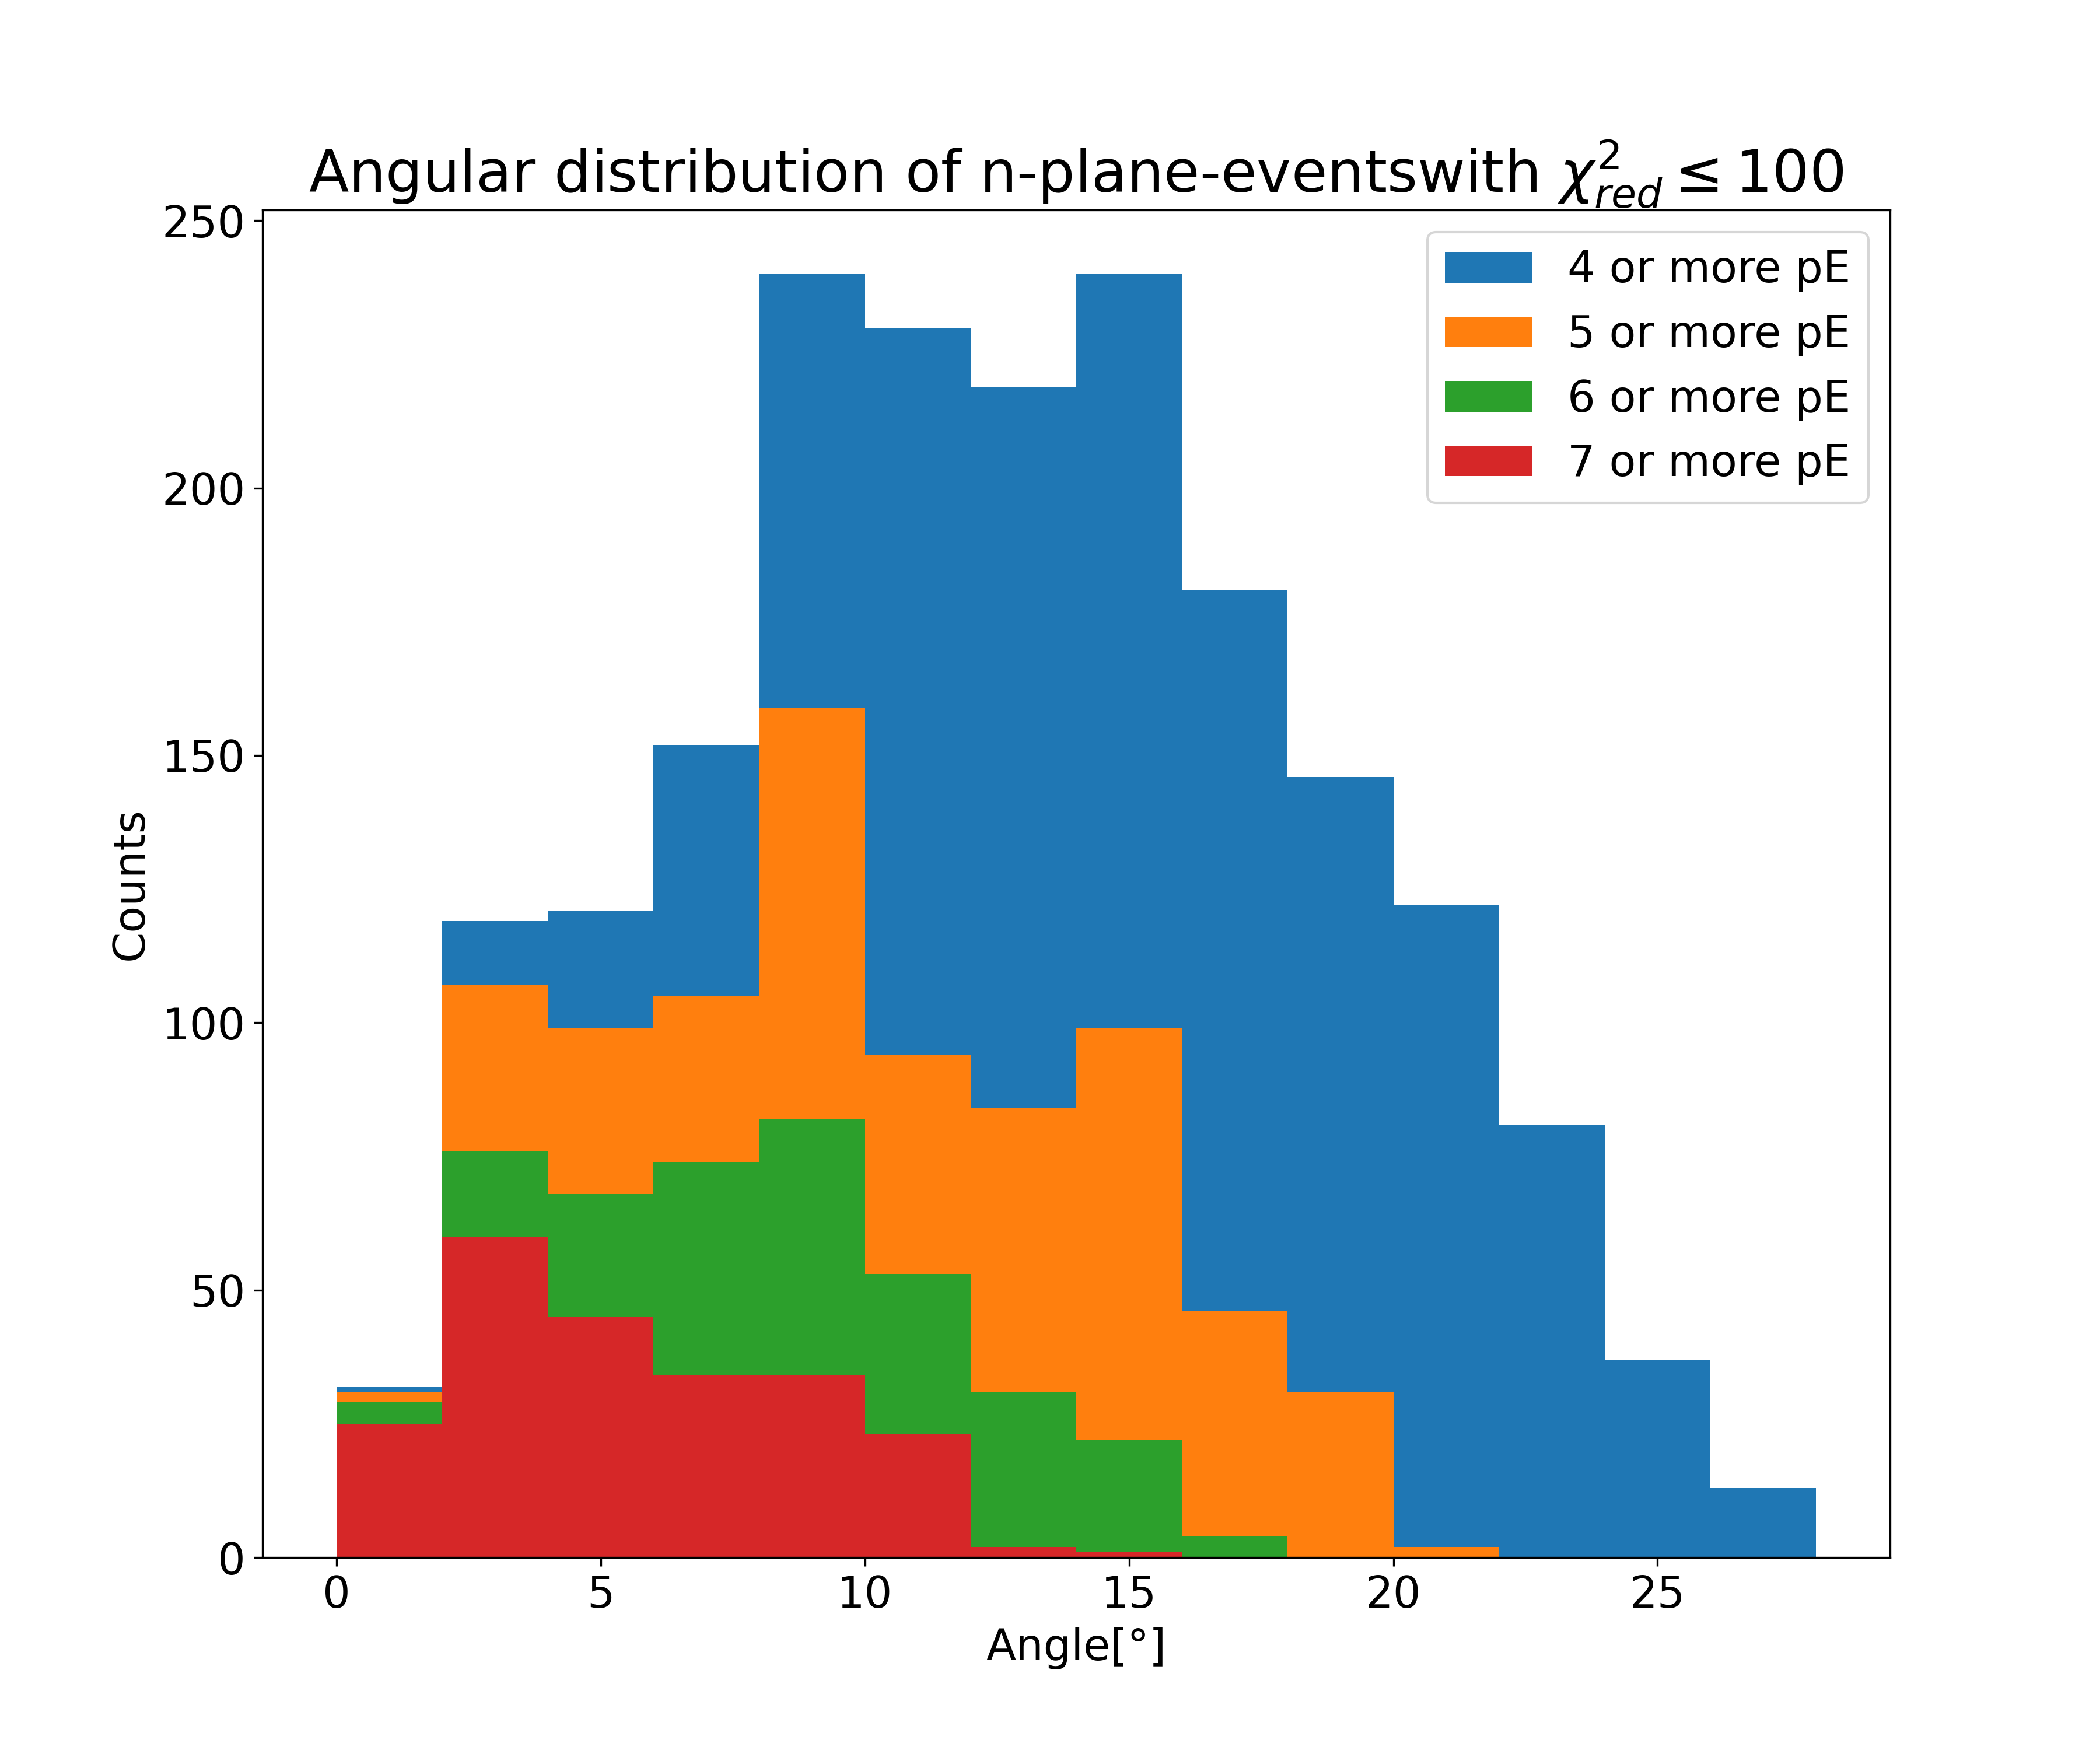
\includegraphics[width=.49\textwidth]{track_angle}
  \end{figure}
\end{frame}

%\begin{frame}{APENDIX}
%  \LARGE Muon rate calculation \normalsize \\[.5cm]
%\end{frame}



\begin{frame}{Outlook}
    \begin{minipage}{.44\textwidth}
	\LARGE Projects \normalsize \\
	\begin{itemize}
	    \item Alignment \\[5pt]
		\begin{itemize} \tiny 
		    \item Trying to achieve better alignment by
			iterative track fitting (similar to corryvreckan)
		\end{itemize}
	    \item Cosmic Analysis for Thesis \\[5pt]
		\begin{itemize} \tiny 
		    \item Comparing angular distribution and rate with
			theoretical calculations
		    \item Cluster sizes and cluster analysis
		\end{itemize}
	    \item The ALPIDE-Telescope \\[5pt]
		\begin{itemize} \tiny 
		    \item Now have scintillators again
		    \item Trying to revive the setup in triggered mode
		       	(now together)
		    \item As of right now: Eudaq not able to work with low
			particle rate (maybe you have some input?)
		\end{itemize}
	\end{itemize}
    \end{minipage}
    \begin{minipage}{.55\textwidth}
	\begin{figure}[H]
	    \centering
	    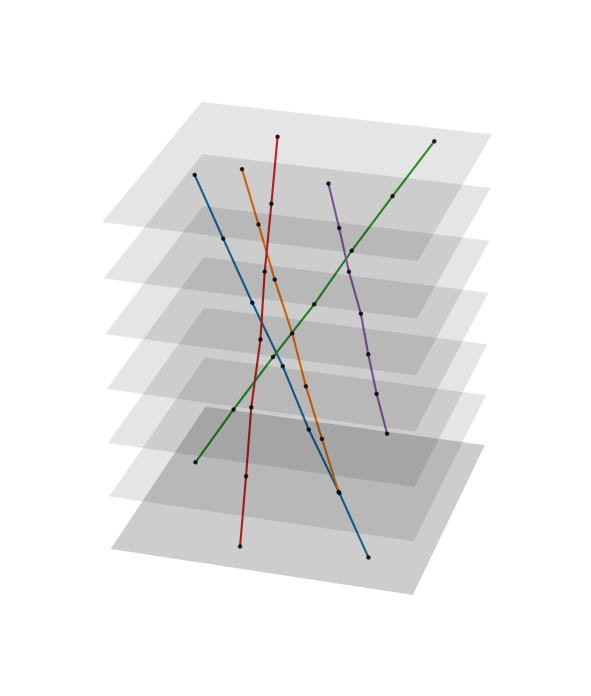
\includegraphics[width=\textwidth]{outlook.png}
	\end{figure}
    \end{minipage}
\end{frame}
\begin{frame}{APENDIX}
  \LARGE $\chi^2_{red}$ \normalsize \\[.5cm]
  \begin{itemize}
    \item $\chi^2_{red}=\frac{\chi^2}{dof}$
    \item dof = number of measurements - variables of the fit
    \item dof = number of traversed planes - 2 (linear fit)
  \end{itemize}
\end{frame}

\end{document}
